\ifdefined\COMPLETE
\else
\documentclass[11pt]{article}
\usepackage[french, english]{babel}
\usepackage[utf8]{inputenc}
\usepackage{graphicx}
\usepackage{framed}
\usepackage[normalem]{ulem}
\usepackage{amsmath}
\usepackage{amsthm}
\usepackage{amssymb}
\usepackage{amsfonts}
\usepackage{enumerate}
\usepackage{import}
\usepackage[top=1 in,bottom=1in, left=1 in, right=1 in]{geometry}
\usepackage{listingsutf8}
\usepackage{color}
\usepackage{float}
\usepackage{graphicx}
\usepackage{subcaption}
\usepackage[toc,page]{appendix}
\usepackage{multicol}
\usepackage{wrapfig}
\usepackage{sidecap}

\floatstyle{boxed} 
\restylefloat{figure}
\definecolor{mygreen}{rgb}{0,0.6,0}
\definecolor{mygray}{rgb}{0.5,0.5,0.5}
\definecolor{mymauve}{rgb}{0.58,0,0.82}
\newcommand{\dt}{\partial_t}
\newcommand{\Tl}{\frac{T}{\lambda}}
\theoremstyle{definition}
\newtheorem{definition}{Définition}[section]
\DeclareMathOperator*{\argmax}{arg\,max}
\DeclareMathOperator*{\argmin}{arg\,min}
 


\lstset{ 
  backgroundcolor=\color{white},   % choose the background color; you must add \usepackage{color} or \usepackage{xcolor}; should come as last argument
  basicstyle=\footnotesize,        % the size of the fonts that are used for the code
  breakatwhitespace=false,         % sets if automatic breaks should only happen at whitespace
  breaklines=true,                 % sets automatic line breaking
  captionpos=b,                    % sets the caption-position to bottom
  commentstyle=\color{mygreen},    % comment style
  deletekeywords={...},            % if you want to delete keywords from the given language
  escapeinside={\%*}{*)},          % if you want to add LaTeX within your code
  extendedchars=true,              % lets you use non-ASCII characters; for 8-bits encodings only, does not work with UTF-8
  firstnumber=1000,                % start line enumeration with line 1000
  frame=single,	                   % adds a frame around the code
  keepspaces=true,                 % keeps spaces in text, useful for keeping indentation of code (possibly needs columns=flexible)
  keywordstyle=\color{blue},       % keyword style
  language=Python,                 % the language of the code
  morekeywords={*,...},            % if you want to add more keywords to the set
  numbers=left,                    % where to put the line-numbers; possible values are (none, left, right)
  numbersep=5pt,                   % how far the line-numbers are from the code
  numberstyle=\tiny\color{mygray}, % the style that is used for the line-numbers
  rulecolor=\color{black},         % if not set, the frame-color may be changed on line-breaks within not-black text (e.g. comments (green here))
  showspaces=false,                % show spaces everywhere adding particular underscores; it overrides 'showstringspaces'
  showstringspaces=false,          % underline spaces within strings only
  showtabs=false,                  % show tabs within strings adding particular underscores
  stepnumber=2,                    % the step between two line-numbers. If it's 1, each line will be numbered
  stringstyle=\color{mymauve},     % string literal style
  tabsize=2,	                   % sets default tabsize to 2 spaces
  title=\lstname                   % show the filename of files included with \lstinputlisting; also try caption instead of title
}
\lstset{inputencoding=utf8/latin1}
\newcommand{\Dt}{\Delta t}
\newcommand{\Dx}{\Delta x}
 %file containing all the used libraries
\newtheorem{theorem}{Théorème}
\begin{document}
\fi

\section{Simulation de l’équation fluide et confirmation du résultat de convergence de la vitesse d'onde sélectionnée vers la vitesse d'onde $s_-$}

Dans cette partie nous allons expliquer la méthode de simulation de l’équation pour le fluide et le résultat obtenu sur la vitesse de propagation:

\subsection{Schéma Numérique}
On souhaite simuler le système d'équations :
\begin{equation}  \left \{
                \begin{array}{ll}
                \dt\mu + \nabla(\mu v) = f(C)(\mu + \rho) -\mu\rho \\
                   \dt(\mu v)+\nabla(\mu v\times v) +T\nabla\mu=-\lambda\mu v+\mu\nabla C-\mu v \rho \\
                 \dt\rho=  F(v) \mu \\
                  \dt C = -b\rho C.
                \end{array}
              \right.
\end{equation} 
Une simulation numérique eulérienne par splitting de Strang du système à été utilisée:\\ 
Pour la membre de gauche des équations (partie hyperbolique advéctive), on utilise un flux numérique approché. Plusieurs approches ont été tentées : un flux de Roe, un flux de Lax-Friedrichs et un flux WENO. Le flux Lax-Friedrichs a l'avantage d'être entropique et robuste en présence de vide, ce qui est exactement le problème autour du front. En revanche, ce flux est extrêmement diffusif, ce qui pose des problèmes lors de la capture du front. Le flux WENO, bien que basé sur le flux Lax-Friedrichs, est oscillant dans les zones de fort gradient, ce qui donne des densités $\mu$ négatives près du front.
Le flux de Roe est celui qui a été choisi au final et semble bien se comporter, modulo la régularisation suivante près du front:
\begin{equation}
     \left \{ \begin{array}{ll}
\dt \mu + \nabla(\mu v) = f(C)(\mu + \rho) -\mu\rho \\
 \dt(\mu v)+\nabla(\frac{\mu v\times \mu v}{\sqrt{\mu^2 + \epsilon^2}}) +T\nabla\mu=-\lambda\mu v+\mu\nabla C-\mu v \rho 
 \end{array}
 \right.
\end{equation}
La partie de gauche (partie réaction) est ensuite résolue de façon totalement implicite (c'est un système du second degré)
\newpage
\subsection{Convergence de la vitesse du front}

\begin{figure}[h]
\centering
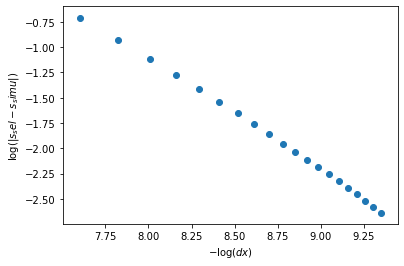
\includegraphics[width=.9\textwidth]{Images/ordrecv_vitessefluide.png}
\caption{Convergence de la vitesse du front observée numériquement}
\end{figure}
La figure ci dessus montre la convergence de la vitesse du front observée numériquement. Ici, $\epsilon=10^{-7}$ et les paramètres physiques sont fixés: 
longueur totale = 1000,
temps total = 100,
$b = .7$,
$F_0 = .8$,
$f_0 = 1$,
$T=10$,
$\lambda =3$.\\
On fait alors varier le pas d'espace $dx$ et on observe l'erreur $|s_{sel}-s_{simu}|$  où $s_{sel}=s_-$ est la vitesse déterminée dans la partie précédente par la condition d'amortissement et $s_{simu}=\frac{X(t_1+t_2)-X(t_1)}{t_2}$ où $t_1$ et $t_2$ sont deux temps arbitraires où le front est déjà établi et $
	 X(t)=\inf(x / \rho(x,t)> \frac{\sup(\rho)}{2}) $ est la position du front.\\
L'ordre de convergence (en fonction pas d'espace $dx$) est alors numériquement 1, ce qui est cohérent avec les méthodes et le schéma utilisé.  
\newpage
\subsection{Sélection de la vitesse minimale d'amortissement}
\begin{figure}[h!]
\centering
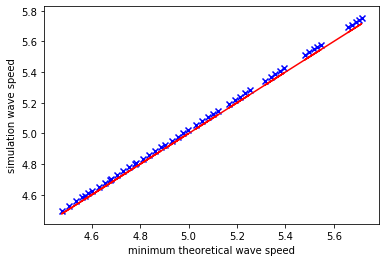
\includegraphics[width=.9\textwidth]{Images/s_sel_fluide.png}
\caption{Vitesse du front observée numériquement en fonction de la vitesse minimale d'amortissement $s_{sel}=s_-$}
\end{figure}


Le graphe ci dessus représente par les points bleus la vitesse du front observée numériquement pour différents paramètres physiques (différents $T$, $\lambda$, $F_0$ et $f_0$) en fonction de la vitesse minimale théorique d'amortissement $s_{sel}=s_-$ associée à cette simulation. \\
La droite rouge est la droite $s_{simu} = s^*_{theorique}$.\\
On remarque encore une fois que la vitesse du front observée numériquement est toujours très proche de la vitesse minimale théorique d'amortissement décrite ci dessus.
\newpage
\subsection{Validation de la condition d'amortissement critique}
Pour certains jeux de paramètres $T$, $\lambda$, $F_0$ et $f_0$, la vitesse $s_{sel} \approx s_{simu}$ ne donne que deux racines réelles au polynôme $A_s$, ce qui confirme que la vitesse de sélection correspond bien a la condition d'amortissement décrite dans la partie ci dessus (régime critique) et non pas le fait que toutes les racines soient réelles (solutions exponentielles décroissantes ou régime apériodique).
\begin{figure}[h!]
\centering
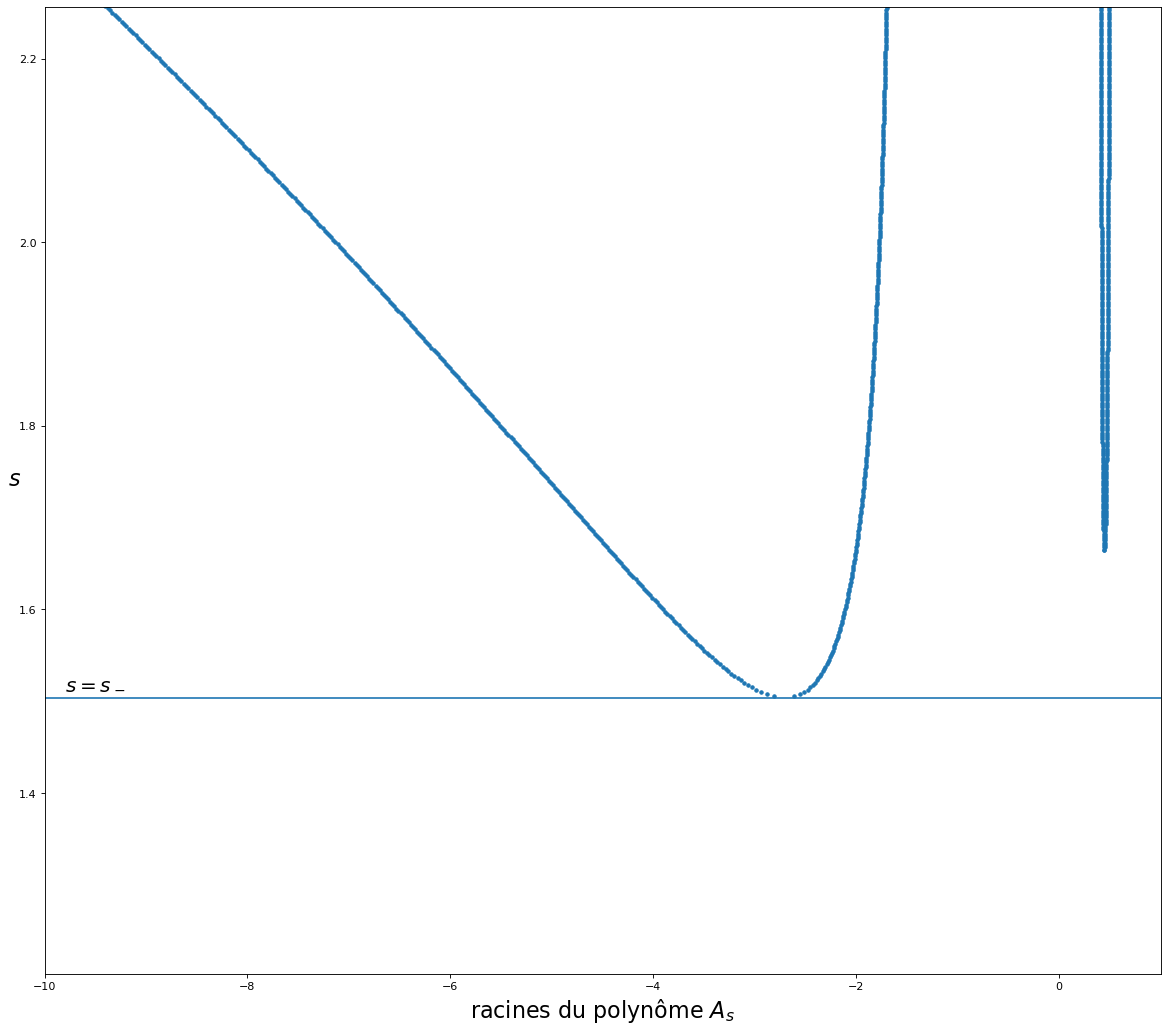
\includegraphics[width=.9\textwidth]{Images/2racines.png}
\caption{Seulement deux racines réelles pour certains jeux de paramètres}
\end{figure}
\ifdefined\COMPLETE
\else
\end{document}
\fi